A natural approach for aggregating an infinite sequence of weights is to consider the arithmetic mean.
Since the sequence $(\frac{1}{k} \sum_{i = 0}^{k-1} \rho_i)_{k \in \N}$ may not converge,
we can either consider the limit superior or the limit inferior, leading to the two definitions:
\[
\MeanPayoff^+(\rho) = \limsup_k \frac{1}{k} \sum_{i = 0}^{k-1} \rho_i \quad ; \quad 
\MeanPayoff^-(\rho) = \liminf_k \frac{1}{k} \sum_{i = 0}^{k-1} \rho_i.
\]
The goal of Eve is to maximise $\MeanPayoff^+$, which means that the goal of Adam is to minimise it, 
or equivalently to maximise $-\MeanPayoff^+$;
by taking the opposite of each weight this is equivalent to maximising $\MeanPayoff^-$.
In other words, $\MeanPayoff^+$ and $\MeanPayoff^-$ are dual objectives.

\vskip1em
In this section we study mean payoff games.
We will first prove that they are prefix independent, then that they are positionally determined for both players,
and then construct algorithms for solving them and compute the value function.
The best known time complexity for both problems is pseudopolynomial, meaning polynomial when the numerical inputs are given in unary.

\begin{lemma}[Prefix independence] 
\label{4-lem:prefix_independence_mean_payoff}
$\MeanPayoff^+$ is prefix independent.
\end{lemma}
\begin{proof}
We show that $\MeanPayoff^+(\rho_0 \rho_1 \dots) = \MeanPayoff^+(\rho_p \rho_{p+1} \dots)$
for a fixed $p \in \N$:
\begin{align*}
\limsup_k \frac{1}{k} \sum_{i = 0}^{k-1} \rho_i &= 
\limsup_k \left(
\underbrace{\frac{1}{k} \sum_{i = 0}^{p-1} \rho_i}_{\rightarrow 0 \text{ for } k \rightarrow \infty} + 
\underbrace{\frac{k-p}{k}}_{\rightarrow 1 \text{ for } k \rightarrow \infty} \cdot \frac{1}{k-p} \sum_{i = p}^{k-1} \rho_i
\right) \\
&=
\liminf_k \frac{1}{k-p} \sum_{i = 0}^{p-1} \rho_{p + i}.
\end{align*} %The same argument holds for $\MeanPayoff^-$.
\end{proof}
Note that by duality this implies that $\MeanPayoff^-$ is also prefix independent.

In the setting we consider in this chapter, meaning two player zero sum games of perfect information, 
the two objectives are equivalent, which will be a corollary of~\cref{4-thm:mean_payoff_positional}.
We refer to~\cref{12-thm:MMP-Eve}\todo{I do not know where this
theorem has disappeared...} for a setting where limit superior and limit inferior are not equivalent.

As an example, consider the mean payoff game represented in~\cref{4-fig:MP}. 
As we will show later, the positional strategies defined below are optimal strategies for Eve and Adam:
\[
\begin{array}{l}
\sigma^*(v_1) = (v_1,v_2) \quad ; \quad \sigma^*(v_3) = (v_3,v_1) \quad ; \quad \sigma^*(v_4) = (v_4,v_0) \\
\tau^*(v_0) = (v_0,v_4) \quad ; \quad \tau^*(v_2) = (v_2,v_3).
\end{array}
\]
Let us consider $\pi = \pi^{v_1}_{\sigma^*,\tau^*}$ the play starting from $v_1$ consistent with both $\sigma^*$ and $\tau^*$:
\[
\pi = \big((v_1,v_2)(v_2,v_3)(v_3,v_1)\big)^\omega.
\]
We obtain that $\MeanPayoff^+(\pi) = \frac{1 + 3 - 2}{3} = \frac{2}{3}$.

If we restrict ourselves to positional strategies for both players, 
we may easily convince ourselves that this is the best that both players can aim for. 
Indeed,
\begin{itemize}
\item the self loop around $v_4$ has arithmetic mean $O$;
\item the simple cycle alternating between $v_0$ and $v_4$ has arithmetic mean $\frac{1}{2}$;
\item the simple cycle alternating between $v_0$ and $v_1$ has arithmetic mean $1$;
\item the self loop around $v_2$ has arithmetic mean $3$, and
\item the simple cycle alternating between $v_0$, $v_1$, $v_2$ and $v_3$ has arithmetic average $\frac{3}{4}$.
\end{itemize}
Eve cannot ensure a better outcome than $\frac{2}{3}$ from $v_1,v_2$, and $v_3$:
for instance if she switches her decision in $v_1$ to play $(v_1,v_0)$, 
she will get a lower outcome of $\frac{1}{2}$.
Similarly Adam cannot ensure a better outcome than $\frac{1}{2}$ from $v_0$ and $v_4$.
Let us now prove that positional strategies are indeed sufficient for mean payoff games.
 
\begin{figure}[tbp]
  \centering
  \begin{tikzpicture}[node distance=2.5cm]
    \node[s-adam](0) {$\begin{array}{c}v_0 \\ 1 \end{array}$};%
    \node[s-eve,below of=0](1) {$\begin{array}{c}v_1 \\ 1 \end{array}$};%
    \node[s-adam,left of=1](2) {$\begin{array}{c}v_2 \\ 3 \end{array}$};%
    \node[s-eve,left of=0](3) {$\begin{array}{c}v_3 \\ -2 \end{array}$};%
    \node[s-eve,right of=0](4) {$\begin{array}{c}v_4 \\ 0 \end{array}$};%

    \path[arrow] 
    (0) edge[bend right=20] (1)%
    (1) edge[bend right=20] (0)%
    (1) edge (2)%
    (2) edge[selfloop=180] (2)%
    (2) edge (3)%
    (3) edge (1)%
    (3) edge (0)%
    (0) edge[bend left=20] (4)%
    (4) edge[bend left=20] (0)
    (4) edge[selfloop=-90] (4);%
  \end{tikzpicture}
\caption{A mean payoff game.}
\label{4-fig:MP}
\end{figure}

%\begin{figure}[tbp]
%  \centering
%  \begin{tikzpicture}[node distance=2.5cm]
%    \node[s-eve](0) {$v_0$};%
%    \node[s-adam,below of=0](1) {$v_1$};%
%    \node[s-eve,left of=1](2) {$v_2$};%
%    \node[s-adam,left of=0](3) {$v_3$};%
%    \node[s-adam,right of=0](4) {$v_4$};%
%
%    \path[arrow] (0) edge[bend right=20] node[left] {4} (1)%
%    (1) edge[bend right=20] node[right] {0} (0)%
%    (1) edge node[below] {2} (2)%
%    (2) edge[selfloop=180] node[left] {1} (2)%
%    (2) edge node[left] {4} (3)%
%    (3) edge node[below left] {$-1$} (1)%
%    (3) edge node[above] {$-2$} (0)%
%    (0) edge[bend left=20] node[above] {$5$} (4)%
%    (4) edge[bend left=20] node[below] {$-2$} (0)
%    (4) edge[selfloop=-90] node[below] {2} (4);%
%  \end{tikzpicture}
%\caption{A mean payoff game.}
%\label{4-fig:MP}
%\end{figure}

\subsection*{Positional determinacy via first cycle games}
\begin{theorem}[Positional determinacy of Mean-Payoff]
\label{4-thm:mean_payoff_positional}
Limit superior mean payoff objectives are uniformly positionally determined for both players.
\end{theorem}
By duality this is equivalent to saying that both limit superior and limit inferior mean payoff objectives are uniformly positionally determined.

\begin{proof}
Let $\arena$ an arena.
We represent a cycle as a sequence $c = v_0 v_1 \dots v_{k-1}$ such that $(v_i, v_{i+1 \mod k}) \in E$;
we note that for technical convenience the sequence does not cycle back to the first vertex.

Let us consider a finite play $\pi = v_0 v_1 v_2\dots$,
we define two objects by induction: 
the cycle decomposition $\Cycles(\pi)$ and the folded play $\widehat{\play}$.
To guide the intuititon: $\Cycles(\pi)$ is a list of \textit{some} cycles in $\pi$, 
and $\widehat{\play}$ is obtained from $\pi$ by removing the cycles from $\Cycles(\pi)$
and does not contain any cycle.

%If $\pi$ is empty then both cycle decomposition and folded play are empty as well.
If $\pi$ is a single vertex then the cycle decomposition is empty and the folded play is equal to $\pi$.
Otherwise let $\pi = \pi' \cdot v$, by induction we have already defined $\Cycles(\pi')$ and $\widehat{\pi'}$.
There are two cases:
\begin{itemize}
	\item Either $v$ appears in $\widehat{\pi'}$ and then $\widehat{\pi}$ is obtained from $\widehat{\pi'} \cdot v$ 
	by replacing that cycle by $v$ and $\Cycles(\pi)$ by adding the cycle to $\Cycles(\pi')$.
%	(Note that since $\widehat{\pi}$ does not contain any cycle, there is at most one cycle in $\widehat{\pi} \cdot v$ and it includes $v$.)
	\item Or $v$ does not appear in $\widehat{\pi'}$ and then $\widehat{\pi} = \widehat{\pi'} \cdot v$ 
	and $\Cycles(\pi) = \Cycles(\pi')$.
\end{itemize}
The cycle decomposition breaks down $\pi$ into (possibly interleaved) cycles and the folded play:
every vertex in $\pi$ either belongs to exactly one cycle in $\Cycles(\pi)$ or to $\widehat{\pi}$.
For instance for $\pi = v_0 v_1 v_2 v_3 v_2 v_4 v_1 v_5$
we have $\Cycles(\pi) = (c_1 = v_2 v_3 ; c_2 = v_1 v_2 v_4)$ and $\widehat{\pi} = v_0 v_1 v_5$,
as illustrated in~\cref{4-fig:example_cycle_decomposition}.

\begin{figure}[!ht]
    \begin{center}
    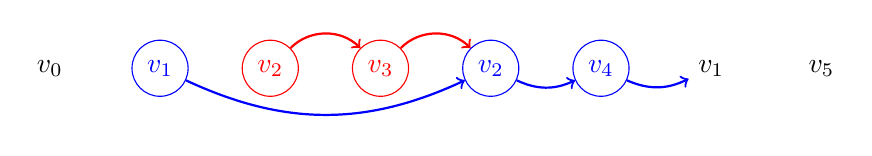
\begin{tikzpicture}
    \tikzstyle{seqc}=[draw, circle]
    \node [] (v0) {$v_0$};
    \node [seqc, blue, right of=v0, node distance=1.4cm] (v1) {$v_1$};
    \node [seqc, red, right of=v1, node distance=1.4cm] (v2) {$v_2$};
    \node [seqc, red, right of=v2, node distance=1.4cm] (v3) {$v_3$};
    \node [seqc, blue, right of=v3, node distance=1.4cm] (v4) {$v_2$};
    \node [seqc, blue, right of=v4, node distance=1.4cm] (v5) {$v_4$};
    \node [right of=v5, node distance=1.4cm] (v6) {$v_1$};
    \node [right of=v6, node distance=1.4cm] (v7) {$v_5$};

    \path[->,thick,bend left=45,red]
        (v2) edge (v3)
        (v3) edge (v4)
        ;

    \path[->,thick,bend right=25,blue]
        (v1) edge (v4)
        (v4) edge (v5)
        (v5) edge (v6)
        ;
    \end{tikzpicture}
    \end{center}
\caption{An example for the cycle decomposition. The first cycle is $c_1$ and is in red, 
the cycle $c_2$ is in blue, and $\widehat{\pi} = v_0 v_1 v_5$.}
\label{4-fig:example_cycle_decomposition}
\end{figure}

%\begin{figure}[!ht]
%    \begin{center}
%    \begin{tikzpicture}
%    \tikzstyle{seqc}=[draw, circle]
%    \node [] (e0) {$(v_0,v_1)$};
%    \node [seqc, blue, right of=e0, node distance=1.4cm] (e1) {$(v_1,v_2)$};
%    \node [seqc, red, right of=e1, node distance=1.4cm] (e2) {$(v_2,v_3)$};
%    \node [seqc, red, right of=e2, node distance=1.4cm] (e3) {$(v_3,v_4)$};
%    \node [seqc, red, right of=e3, node distance=1.4cm] (e4) {$(v_4,v_2)$};
%    \node [seqc, blue, right of=e4, node distance=1.4cm] (e5) {$(v_2,v_5)$};
%    \node [seqc, blue, right of=e5, node distance=1.4cm] (e6) {$(v_5,v_1)$};
%    \node [right of=e6, node distance=1.4cm] (e7) {$(v_6,v_1)$};
%
%    \path[->,thick,bend left=45,red]
%        (e2) edge (e3)
%        (e3) edge (e4)
%        ;
%
%    \path[->,thick,bend right=35,blue]
%        (e1) edge (e5)
%        (e5) edge (e6)
%        ;
%    \end{tikzpicture}
%    \end{center}
%\caption{An example for the cycle decomposition. The first cycle is $c_1$ and is in red, 
%the cycle $c_2$ is in blue, and the other two edges form $\widehat{\pi}$.}
%\label{4-fig:example_cycle_decomposition}
%\end{figure}

The definition of $\Cycles(\pi)$ is extended for infinite plays.
We write $\FC(\pi)$ for the first cycle in $\pi$.
Let us note that the definitions above do not depend on the mean payoff objectives.

Let $\game = (\arena,\MeanPayoff^+[\col])$ a limit superior mean payoff game.
The outline of the proof is as follows.
\begin{enumerate}
	\item We define the condition $\FirstCycle$ and $\game_{\text{FC}} = (\arena,\FirstCycle)$,
	and show that $\val^{\game} = \val^{\game_{\text{FC}}}$ 
	and that if $\game_{\text{FC}}$ is positionally determined for both players then $\game$ is positionally determined for both players.
	\item We define the condition $\FirstCycleReset_v$ (parameterised by a vertex $v$) 
	and $\game_{\text{FCR}(v)} = (\arena,\FirstCycleReset_v)$,
	and show that $\val^{\game} = \val^{\game_{\text{FCR}(v)}}$.
	\item We show that $\game_{\text{FC}}$ is positionally determined for both players.
\end{enumerate}

\vskip1em
\textbf{Step 1.}
For a path $\pi = v_0 v_1 \dots v_{k-1}$ we write $\Mean(\pi)$ for $\frac{1}{k} \sum_{i = 0}^{k-1} \col(v_i)$.
The condition $\FirstCycle$ computes the arithmetic mean of the first cycle.
Formally:
\[
\FirstCycle(\pi) = \Mean(\FC(\pi)).
\]
Let us define $\game_{\text{FC}} = (\arena,\FirstCycle)$.
We make two claims:
\begin{itemize}
	\item let $\sigma_{\text{FC}}$ a strategy in $\game_{\text{FC}}$, it induces a strategy $\sigma$ in $\game$ 
	such that $\val^{\sigma_{\text{FC}}} \le \val^{\sigma}$, and $\sigma$ is positional if $\sigma_{\text{FC}}$ is, and
	\item let $\tau_{\text{FC}}$ a strategy in $\game_{\text{FC}}$, it induces a strategy $\tau$ in $\game$
	such that $\val^{\tau_{\text{FC}}} \ge \val^{\tau}$, and $\tau$ is positional if $\tau_{\text{FC}}$ is.
\end{itemize}

Let us prove the first claim.
We let $\sigma(\pi) = \sigma_{\text{FC}}(\widehat{\pi})$:
by definition if $\pi$ is a play consistent with $\sigma$ then $\widehat{\pi}$ is a play consistent with $\sigma_{\text{FC}}$.
Note that indeed if $\sigma_{\text{FC}}$ is positional then so is $\sigma$.
We show that $\val^{\sigma_{\text{FC}}} \le \val^{\sigma}$.

Let $\pi$ be a play consistent with $\sigma$ from $v_0$ and $x = \val^{\sigma_{\text{FC}}}(v_0)$.
We first argue that all cycles in $\Cycles(\pi)$ have an arithmetic mean greater than or equal to $x$.
Indeed consider a cycle $c$ in $\Cycles(\pi)$ and let $\pi'$ the prefix of $\pi$
ending with the cycle $c$.
The play $\widehat{\pi'}$ is consistent with $\sigma_{\text{FC}}$, implying that $\Mean(c) \ge x$.

To conclude that $\MeanPayoff^+(\pi) \ge x$ we show the following property:
\begin{equation}\label{4-eq:cycle_positive}
(\forall c \in \Cycles(\pi),\ \Mean(c) \ge x) \implies \MeanPayoff^+(\pi) \ge x.
\end{equation}

To estimate $\MeanPayoff^+(\pi)$ let us look at the prefix $\pi_{< k}$ of $\pi$ of length $k$.
Indeed we note that $\MeanPayoff^+(\pi) = \limsup_k \Mean(\pi_{< k})$.

To calculate $\Mean(\pi_{< k})$ we use the fact that 
every vertex in $\pi_{< k}$ either belongs to exactly one cycle in $\Cycles(\pi_{< k})$ or to $\widehat{\pi_{< k}}$,
and the linearity of the arithmetic mean: 
\[
\Mean(\pi_{< k}) = \Mean \set{\Mean(\widehat{\play_{< k}}), \set{\Mean(c) : c \in \Cycles(\pi_{< k})}}.
\]
By assumption each $\Mean(c)$ is greater than or equal to $x$.
Note that since $\widehat{\play_{< k}}$ does not contain any cycle, it has length at most $n$, independently of $k$.
On the other hand $\Cycles(\pi_{< k})$ has size at least $k / n$.
Hence when $k$ tends to infinity the term $\Mean(\widehat{\play_{< k}})$ vanishes and we have 
$\MeanPayoff^+(\pi) = \limsup_k \Mean(\pi_{< k}) \ge x$.

\vskip1em
We turn to the second claim.
The construction is identical for Adam:
we let $\tau(\pi) = \tau_{\text{FC}}(\widehat{\pi})$.
We show that $\val^{\tau_{\text{FC}}} \ge \val^{\tau}$ following the same arguments.
Let $\pi$ be a play consistent with $\tau$ from $v_0$ and $x = \val^{\tau_{\text{FC}}}(v_0)$.

To conclude that $\MeanPayoff^+(\pi) \le x$ we show the following property:
\begin{equation}\label{4-eq:cycle_negative}
(\forall c \in \Cycles(\pi),\ \Mean(c) \le x) \implies \MeanPayoff^+(\pi) \le x.
\end{equation}
This follows as above from the linearity of the arithmetic mean and the cycle decomposition.
%To get the strict inequality we additionally observe that there are finitely different cycles in $\Cycles(\pi_{< k})$,
%independently of $k$, since they are simple cycles hence of length at most $n$.
%So the assumption can be strengthened to: there exists $\varepsilon > 0$ 
%such that all cycles $c$ in $\Cycles(\pi)$ satisfy $\Mean(c) \le x - \varepsilon$.
%Then we obtain that $\MeanPayoff^+(\pi) \le x - \varepsilon < x$.

\vskip1em
Let us now prove that $\val^{\game} = \val^{\game_{\text{FC}}}$ using the two claims.
We first need to establish that $\game_{\text{FC}}$ is determined: 
one argument is that $\FirstCycle$ is a Borel condition, 
hence determinacy follows from the general Borel determinacy result (\cref{1-thm:borel_determinacy}),
another simpler argument is that $\FirstCycle$ is a finite duration condition,
meaning that the outcome of the play is determined with a finite number of steps (at most $n$),
hence determinacy follows from an easier direct argument for finite duration games.

It follows from the two claims that 
\[
\begin{array}{llll}
\val^{\game_{\text{FC}}} 
& = \sup_{\sigma_{\text{FC}}} \val^{\sigma_{\text{FC}}} 
& \le \sup_{\sigma} \val^{\sigma}
& = \val^{\game} \\
\val^{\game_{\text{FC}}}
& = \inf_{\tau_{\text{FC}}} \val^{\tau_{\text{FC}} }
& \ge \inf_{\tau} \val^{\tau}
& = \val^{\game},
\end{array}
\]
where in both lines: 
the first equalities is by determinacy of $\game_{\text{FC}}$,
the inequalities thanks to the two claims,
and the last equalities by determinacy of $\game$.
The two obtained inequalities imply that $\val^{\game} = \val^{\game_{\text{FC}}}$,
and positional optimal strategies for either player in $\game_{\text{FC}}$ 
induce positional optimal strategies in $\game$.

\vskip1em
\textbf{Step 2.}
We define a third condition on $\arena$:
\[
\FirstCycleReset_v(\pi) = 
\begin{cases}
\FirstCycle(\pi) & \text{ if } \pi \text{ does not visit } v \text{ before } \FC(\pi), \\
\FirstCycle(\pi_{\ge k}) & \text{ for } k \text{ the first index such that } \Ing(\pi_k) = v.
\end{cases}
\]
In words: if a cycle is closed before visiting $v$, then the condition is $\FirstCycle$
and otherwise when reaching $v$ the game is ``reset'' and the condition is $\FirstCycle$ from this point onwards.

This second step is similar to the first step; the reason why we separated them is because this step
relies on the fact that $\MeanPayoff^+$ is "prefix independent".

Let us define $\game_{\text{FCR}(v)} = (\arena,\FirstCycleReset_v)$.
We make two claims:
\begin{itemize}
	\item let $\sigma_{\text{FCR}(v)}$ an optimal strategy in $\game_{\text{FCR}(v)}$, it induces a strategy $\sigma$ in $\game$ 
	such that $\val^{\sigma_{\text{FCR}(v)}} \le \val^{\sigma}$, and 
	\item let $\tau_{\text{FCR}(v)}$ an optimal strategy in $\game_{\text{FCR}(v)}$, it induces a strategy $\tau$ in $\game$
	such that $\val^{\tau_{\text{FCR}(v)}} \ge \val^{\tau}$.
\end{itemize}

Let us prove the first claim.
We let 
\[
\sigma(\pi) = 
\begin{cases}
\sigma_{\text{FCR}(v)}(\widehat{\pi}) & \text{if } \pi \text{ does not contain } v, \\
\sigma_{\text{FCR}(v)}(\widehat{\pi_{\ge k}}) & \text{for } k \text{ the first index such that } \Ing(\pi_k) = v.
\end{cases}
\]
We show that $\val^{\sigma_{\text{FCR}(v)}} \le \val^{\sigma}$.
Let $\pi$ a play consistent with $\sigma$ from $v_0$ and $x = \val^{\sigma_{\text{FCR}(v)}}(v_0)$.
There are two cases.

Either $\pi$ does not contain $v$, and then as in the first step 
this implies that all cycles in $\pi$ have an arithmetic mean greater than or equal to $x$,
and we conclude as in the first step that $\FirstCycleReset_v(\pi) \ge x$.

Or $\pi$ contains $v$. We first argue that $x = \val^{\sigma_{\text{FCR}(v)}}(v_0) \le \val^{\sigma_{\text{FCR}(v)}}(v)$.
Indeed, let $\pi_0$ be a play without cycles from $v_0$ to $v$ consistent with $\sigma_{\text{FCR}(v)}$,
we let $\sigma'(\pi) = \sigma_{\text{FCR}(v)}(\pi_0 \pi)$.
Then $\val^{\sigma_{\text{FCR}(v)}}(v_0) \le \val^{\sigma'}(v) \le \val^{\sigma_{\text{FCR}(v)}}(v)$,
the first inequality is because a play $\pi$ consistent with $\sigma'$ from $v$ 
correspond to the play $\pi_0 \pi$ consistent with $\sigma_{\text{FCR}(v)}$ from $v_0$,
and the second inequality by optimality of $\sigma_{\text{FCR}(v)}$.

Let $y = \val^{\sigma_{\text{FCR}(v)}}(v)$, the inequality above reads $x \le y$.
Let $\pi'$ the suffix of $\pi$ starting from the first occurrence of $v$,
then $\pi'$ is consistent with $\sigma_{\text{FCR}(v)}$ from $v$,
so as in the first step this implies that all cycles in $\pi'$ have an arithmetic mean greater than or equal to $y$.
We conclude as in the first step that $\MeanPayoff^+(\pi') \ge y \ge x$,
The last but important argument is that $\MeanPayoff^+$ is "prefix independent",
implying that $\MeanPayoff^+(\pi) \ge x$.

\vskip1em
We prove that $\val^{\game} = \val^{\game_{\text{FCR}(v)}}$ using the two claims
following the same arguments as in the first step.
In particular we need to establish that $\game_{\text{FCR}(v)}$ is determined,
and again it either follows from the general Borel determinacy result (\cref{1-thm:borel_determinacy})
or by determinacy for finite duration games.

\vskip1em
\textbf{Step 3.}
We (finally!) prove that $\game_{\text{FC}}$ is positionally determined for both players.
Let us prove positional determinacy for Eve, the case of Adam being symmetric.
We show that for all games there exists an optimal positional strategy,
by induction on the number of vertices of Eve with more than one outgoing edge.
The base case is clear since in that case there is a unique strategy and it is positional.
Let $v \in \VE$ with more than one outgoing edge.

Let $\sigma_{\text{FCR}(v)}$ an optimal strategy in $\game_{\text{FCR}(v)}$.
Intuitively, since the game is reset at the first visit of $v$ and that the second visit to $v$ would close a loop hence determine the outcome, 
we can use any optimal strategy from $v$.
We define $\sigma'$ as follows:
\[
\sigma'(\pi) = 
\begin{cases}	
\sigma(\pi) & \text{if } \pi \text{ does not contain } v, \\
\sigma(\pi_{\ge k}) & \text{for } k \text{ the last index such that } \Ing(\pi_k) = v.
\end{cases}
\]
Note that indeed $\sigma'$ uses only one outgoing edge of $v$.
We show that $\val^{\game_{\text{FCR}(v)},\sigma}(v_0) \le \val^{\game_{\text{FCR}(v)},\sigma'}(v_0)$,
implying that $\sigma'$ is optimal in $\game_{\text{FCR}(v)}$ and the inequality is an equality.

Let $\pi$ be a play consistent with $\sigma'$ from $v_0$.
If it does not contain $v$ it is consistent with $\sigma$, so $\FirstCycleReset_v(\pi) \ge \val^{\game_{\text{FCR}(v)},\sigma}(v_0)$.
If it contains $v$, let $\pi'$ the suffix of $\pi$ starting from the first occurrence of $v$,
then $\FirstCycleReset_v(\pi) = \FirstCycle(\pi')$.
Since $\pi'$ is consistent with $\sigma$ (until a cycle is formed) we have $\FirstCycle(\pi') \ge \val^{\game_{\text{FCR}(v)},\sigma}(v_0)$,
implying that $\FirstCycleReset_v(\pi) \ge \val^{\game_{\text{FCR}(v)},\sigma}(v_0)$.
We conclude: $\val^{\game_{\text{FCR}(v)},\sigma'}(v_0) \le \val^{\game_{\text{FCR}(v)},\sigma}(v_0)$.

Let $\mathcal{B}$ the arena obtained from $\arena$ by removing all outgoing edges of $v$ not used by $\sigma'$.
Let $\game'_{\text{FCR}(v)} = (\mathcal{B}, \FirstCycleReset_v)$ and $\game'_{\text{FC}} = (\mathcal{B}, \FirstCycle)$.
By definition we have $\val^{\game_{\text{FCR}(v)},\sigma'} = \val^{\game'_{\text{FCR}(v)},\sigma'} = \val^{\game'_{\text{FCR}(v)}}$.
In the previous step we proved that $\val^{\game'_{\text{FC}}} = \val^{\game'_{\text{FCR}(v)}}$,
so $\val^{\game'_{\text{FC}}} = \val^{\game_{\text{FC}}}$.
The arena $\mathcal{B}$ contains one less vertex of Eve with more than one outgoing edge,
so the induction hypothesis applies and implies that there exists an optimal strategy in $\game'_{\text{FC}}$,
which is also optimal in $\game_{\text{FC}}$ thanks to the equality $\val^{\game'_{\text{FC}}} = \val^{\game_{\text{FC}}}$.
\end{proof}

%Before drawing corollaries from this result, 
Let us extract from the proof of~\cref{4-thm:mean_payoff_positional} a more general positionality result via first cycle games.

\begin{theorem}[Generalised positional determinacy]
\label{4-thm:first_cycle_games}
Let $\Phi$ a quantitative objective over the set of colours $C$.
Let $f : C^* \to \R$ satisfying the following properties,
for all games $\Game$ with objective $\Phi$:
\begin{itemize}
	\item for all $x \in \Rinfty$, for all plays $\pi$, 
	\[
	(\forall c \in \Cycles(\pi),\ f(c) \ge x) \implies \Phi(\pi) \ge x,
	\]
	\item for all $x \in \Rinfty$, for all plays $\pi$, 
	\[
	(\forall c \in \Cycles(\pi),\ f(c) \le x) \implies \Phi(\pi) \le x,
	\]
	\item $\Phi$ is prefix independent.
%	\item for all $\rho,\rho' \in C^*$ we have $f(\rho \rho') = f(\rho' \rho)$.
\end{itemize}
Then $\Phi$ is positionally determined for both players.
\end{theorem}
In the proof above, the role of $f$ is played by the function $\Mean$.

The first two items are used to prove that the first cycle games induced by $f$ are equivalent to the games with objective $\Phi$,
and the third item to prove the equivalence with first cycle games with reset;
the equivalence between the two types of first cycle games yield the positionality of these games,
implying the positionality of games with objective $\Phi$.

\begin{corollary}[Limit superior and limit inferior mean payoff games]\hfill
\label{4-cor:rational-MP}
\begin{itemize}
	\item Limit superior and limit inferior mean payoff games are equivalent:
	for every arena $\arena$ and colouring function $\col : E \to \Z$,
	let $\game_{+} = (\arena,\MeanPayoff^+[\col])$ and $\game_{-} = (\arena,\MeanPayoff^-[\col])$,
	then $\val^{\game_+} = \val^{\game_-}$.
	This implies that a positional strategy is optimal in $\game_+$ if and only if it is optimal in $\game_-$.
	
	Since they are equivalent we speak of mean payoff games without specifying whether the objective is $\MeanPayoff^+$ or $\MeanPayoff^-$,
	and write $\MeanPayoff$ instead.

	\item For all mean payoff games $\game$ and vertices $v$, 
	the value $\Value^\game(v)$ is a rational number of the form $\frac{a}{n}$ with $a \in [-nW,nW]$,
	where $W$ is the largest weight appearing in $\Game$ in absolute value.
\end{itemize}
\end{corollary}
\begin{proof}
Thanks to \cref{4-thm:mean_payoff_positional}, there exist $\sigma_+$ and $\tau_+$ optimal positional strategies in $\game_+$
and $\sigma_-$ and $\tau_-$ optimal positional strategies in $\game_-$ (for the latter by duality).
By definition $\val^{\game_+}(v) = \MeanPayoff^+(\pi^v_{\sigma_+,\tau_+})$ and $\val^{\game_-}(v) = \MeanPayoff^-(\pi^v_{\sigma_-,\tau_-})$.
Since $\MeanPayoff^- \le \MeanPayoff^+$ we already have $\val^{\game_-} \le \val^{\game_+}$.

For two positional strategies $\sigma$ and $\tau$, the play $\pi^v_{\sigma,\tau}$ is a lasso, meaning of the form $\pi c^\omega$
with $\pi$ a simple path and $c$ a simple cycle, 
implying that $\MeanPayoff^+(\pi^v_{\sigma,\tau}) = \MeanPayoff^-(\pi^v_{\sigma,\tau})$,
let us write $\MeanPayoff(\pi^v_{\sigma,\tau})$ for this value.

We have:
\[
\MeanPayoff(\pi^v_{\sigma_+,\tau_+}) 
\le \MeanPayoff(\pi^v_{\sigma_+,\tau_-})
\le \MeanPayoff(\pi^v_{\sigma_-,\tau_-}),
\]
where the first inequality is by optimality of $\tau_-$ and the second inequality by optimality of $\sigma_-$.
Hence $\val^{\game_+} \le \val^{\game_-}$, and finally $\val^{\game_+} = \val^{\game_-}$.

\vskip1em
For the second item, recall that $\val^\game(v) = \MeanPayoff(\pi^v_{\sigma,\tau})$
with $\sigma$ and $\tau$ optimal positional strategies.
Let us write $\pi^v_{\sigma,\tau} = \pi c^\omega$ with $\pi$ a simple path and $c$ a simple cycle, 
then by prefix independence $\MeanPayoff(\pi^v_{\sigma,\tau}) = \Mean(c)$,
thus $\val^\game(v)$ is the mean of at most $n$ weights from $\game$.
\end{proof}

\subsection*{\texorpdfstring{Solving mean payoff games in $\NP\cap\coNP$}{Solving mean payoff games in NP and coNP}}
The positional determinacy of mean payoff games easily gives an upper bound on the complexity of \emph{solving} these games.

\begin{theorem}[Complexity of mean payoff]
\label{4-thm:MP-NPcoNP}
Solving mean payoff games is in $\NP\cap\coNP$.
\end{theorem}
\begin{proof}
The first ingredient for this proof is a polynomial time algorithm for solving the one player variants of mean payoff games.
Indeed, they correspond to the minimum cycle mean problem in a weighted graph,
which can be solved in polynomial time by a dynamic programming algorithm.
The second ingredient is the positional determinacy result proved in~\cref{4-thm:mean_payoff_positional}.

Let us show the $\NP$ membership. 
Consider a mean payoff game $\Game$, a vertex $v$ and a threshold~$x \in \Qinfty$.
Thanks to~\cref{4-thm:mean_payoff_positional}, we know that there exist an optimal positional strategy for Eve.
With a non-deterministic Turing machine, we may guess a positional strategy for Eve, and check that it ensures $x$ in $\Game$ from $v$. 

Let us now show the $\coNP$ membership. 
By determinacy of mean payoff games, whether Eve \emph{cannot} ensure $x$ in $\Game$ from $v$ 
is equivalent to whether Adam can ensure $x$ in $\Game$ from $v$.
Again thanks to~\cref{4-thm:mean_payoff_positional}, we know that there exist an optimal positional strategy for Adam.
With a non-deterministic Turing machine, we may guess a positional strategy for Adam, and check that it ensures $x$ in $\Game$ from $v$. 
\end{proof}

We can turn the non-deterministic algorithm given in~\cref{4-thm:MP-NPcoNP} into a deterministic algorithm 
with exponential complexity since there are exponential many positional strategies.

We now show that solving mean payoff games is at least as hard as solving parity games.

\begin{theorem}[Link with parity games]
\label{4-thm:parity2MP}
  Solving parity games reduce in polynomial time to solving mean payoff games with threshold $0$.
\end{theorem}
\begin{proof}
Let $\game = (\arena, \Parity[\col])$ a parity game with $n$ vertices and priorities in $[1,d]$.
We construct a mean payoff game $\game' = (\arena, \MeanPayoff[\col'])$ using the same arena:
\[
\col'(v) = (-n)^{\col(v)}.
\]
Note that $\col'(v)$ is of polynomial size since $\log(|\col'(v)|) = \col(v) \log(n) \leq d \log(n)$.

The key property relating $\col'$ and $\col$ is the following:
for $c = v_0 \dots v_{k-1}$ a simple cycle (implying $k \le n$),
the largest priority in $c$ is even %(meaning $\max \set{\col(v_i) : i \in [0,k-1]}$ is even)
if and only if $\Mean(c) \ge 0$.
Indeed, if the largest priority in $c$ is $p$ even reached in $v_i$ then $\col'(v_i) = n^p$
and for $j \neq i$ we have $\col'(v_j) \ge -n^{p-1}$,
and since there are at most $n$ vertices in total the largest priority dominates the others.

\vskip1em
We claim that $\WE(\game) = \WE(\game')$.

Let $\sigma$ be a positional strategy winning from $\WE(\game)$, we show that $\sigma$ is also winning from $\WE(\game)$ in $\Game'$.
Since mean payoff are uniformly positionally determined for both players (see~\cref{4-thm:mean_payoff_positional}),
there exists $\tau$ a positional strategy winning from $\WA(\game')$.
Let $v \in \WE(\game)$, we consider $\pi = \pi^v_{\sigma,\tau}$ the play consistent with $\sigma$ and $\tau$ starting from $v$.
Since $\sigma$ and $\tau$ are positional, $\pi$ is a simple path followed by a simple cycle $c$.
Because $\sigma$ is winning the largest priority in $c$ is even, 
so thanks to the property above $\Mean(c) \ge 0$, meaning that $\MeanPayoff(\pi) \ge 0$.
Thus $\WE(\game) \subseteq \WE(\game')$.
The converse implication is proved similarly swapping the two players.
%  Starting from a parity game $\game = (\arena, \Parity)$ and a
%  particular starting vertex $v_0\in V$, we build a mean payoff game
%  $\game_{\text{FC}} = (\arena',\MeanPayoff)$ such that Eve has a winning
%  strategy from $v_0$ in $\game$ if and only if Eve can guarantee a
%  mean payoff at least 0 in $\game_{\text{FC}}$. Arena $\arena'$ has the same
%  vertices and edges as $\arena$, but the cost of edges are adapted:
%  letting $r$ be the maximal parity in $\arena$, the new cost function
%  for~$\arena'$ is~$c'$ defined by $c'(e)= (-n)^{c(e)}$ for every
%  edge $e\in E$. Notice that $c'(e)$ is indeed of polynomial size
%  since $\log |c'(e)| = c(e)\log n \leq n\log n$ (the latter
%  holds because we can limit ourselves to parities bounded by the
%  number of vertices in a parity game, without loss of generality).
%
%  Strategies of both players are the same in $\game$ and
%  $\game_{\text{FC}}$. Consider then $\sigma$, a positional strategy of Eve. For
%  every simple cycle $\play$ following strategy $\sigma$, the highest
%  priority of a vertex on $c$ in $\game$ is even if and only if the
%  sum of the weights of the edges on $c$ in $\game_{\text{FC}}$ is
%  nonnegative. For instance, consider a simple cycle with priorities
%  $2$, $3$ and $1$, in a game with $n$ vertices: then the
%  corresponding cycle in $\game_{\text{FC}}$ has cumulated weight
%  $n^2-n^3-n<0$. If the simple cycle has priorities $2$, $0$ and $1$
%  instead, the sum of weights would become $n^2+1-n\geq 0$.
%
%  Moreover, if $\sigma$ is winning for Eve from $v_0$ in~$\game$, then
%  for every simple cycle $c$ following strategy $\sigma$ in $\game$,
%  the highest priority of a vertex appearing on $c$ is even: otherwise
%  Adam can force the play from $v_0$ to $c$ and stay in $c$ forever,
%  and thus win. Similarly, if $\sigma$ is winning for Eve from $v_0$
%  in $\game_{\text{FC}}$, for every simple cycle $c$ following strategy $\sigma$
%  in $\game_{\text{FC}}$, the sum of the weights of the edges on $c$ is
%  nonnegative. By a similar decomposition of an infinite play into
%  simple cycles as the one used in the determinacy proof
%  of~\cref{4-thm:mean_payoff_positional}, we may then show easily that a
%  positional strategy $\sigma$ is winning in $\game$ from $v_0$ if and
%  only if it guarantees to Eve a mean payoff at least $0$ in $\game_{\text{FC}}$.
\end{proof}

We note that we did not construct a reduction between objectives as defined in~\cref{1-sec:reductions}:
indeed it is not true that $\Parity$ reduces to $\MeanPayoff_{\ge 0}$, the reduction depends on the number $n$ of vertices.

As a corollary of~\cref{4-thm:MP-NPcoNP}, this polynomial reduction gives an alternative proof of the fact
that solving parity games is in $\NP \cap \coNP$.

\subsection*{A strategy improvement algorithm}
\begin{theorem}[Strategy improvement algorithm]
\label{4-thm:strategy_improvement}
There exists a strategy improvement algorithm for solving mean payoff games in \mynote{FILL IN}.
\end{theorem}

We rely on the high-level presentation of strategy improvement algorithms given in \cref{1-sec:strategy_improvement}.
The algorithm is very similar and actually extends the strategy improvement algorithm for parity games presented in~\cref{3-sec:strategy_improvement}.

\paragraph{\bf Adding the option of stopping the game.}
Let $\game$ be a mean payoff game with weights in $[-W,W]$.
Let us give Eve an extra move $\siblank$ that indicates that the game should stop and that she can play from any vertex of hers.
So a strategy for Eve is now a function $\sigma : \VE \rightarrow E \cup \set{\siblank}$ 
where $\sigma(v) = \siblank$ indicates that Eve has chosen to stop the game, and $\sigma(v) \ne \siblank$ should be interpreted as normal.
Adam is not allowed to stop the game, so strategies for Adam remain unchanged.
We say that a play ending with $\siblank$ is stopped.

For reasoning it will be useful to consider the mean payoff graph $\Game[\sigma]$ obtained from $\Game$ by restricting the outgoing edges from $\VE$
to those prescribed by $\sigma$. 
We say that a mean payoff graph (without stopping option) ""satisfies"" mean payoff from $v$ if all infinite paths $\pi$ from $v$ satisfy 
$\MeanPayoff(\pi) \ge 0$.
Then a strategy $\sigma$ is winning from $v$ if and only if the mean payoff graph $\Game[\sigma]$ satisfies mean payoff from $v$.

Since we added the option for Eve to stop the game we introduce a new terminology: 
we say that a strategy $\sigma$ ""respects"" mean payoff if all infinite plays consistent with $\sigma$ satisfy mean payoff,
equivalently all infinite paths in $\Game[\sigma]$ satisfy mean payoff, not requiring anything of stopped plays.

We say that a cycle is non-negative if the sum of the weights in the cycle is non-negative, and it is negative otherwise. 
Respecting mean payoff is characterised using cycles:
\begin{fact}[Characterisation using cycles]\label{4-fact:characterisation}
A strategy $\sigma$ ""respects"" mean payoff if and only if all cycles in $\Game[\sigma]$ are non-negative.
\end{fact}
The algorithm will only manipulate strategies respecting mean payoff.

\paragraph{\bf Evaluating a strategy.}
The first question is: given a strategy $\sigma$, how to evaluate it (in order to later improve it)?
As explained in \cref{1-sec:strategy_improvement} towards this goal we define a value function $\val^{\sigma} : V \to Y$.

We let $\val^{\sigma}(v) = \min_\tau \val(\play_{\sigma,\tau}^v)$ where $\tau$ ranges over (general) strategies for Adam, so we first need to define the value of the play $\play = \play_{\sigma,\tau}^v$.
If $\play$ is stopped, then $\val(\play)$ is the sum of the weights in $\play$.
Otherwise $\val(\play)$ is $\top$ if $\play$ satisfies mean payoff, and $\bot$ if $\play$ does not satisfy mean payoff.
So the value of a play is either $\top$, $\bot$, or an integer;
we let $Y = \Zinfty$ and equip it with the natural order $\le$.

\paragraph{\bf The value function as a fixed point.}
We define $\delta : Y \times [-W,W] \to Y$ by 
\[
\delta(t,w) = 
\begin{cases}
t + w & \text{ if } t \in \Z, \\
\top & \text{ if } t = \top, \\
\bot & \text{ if } t = \bot.
\end{cases}
\]
We note that $\delta$ is monotonic: for all $w \in Y$,
if $t \le t'$ then $\delta(t,w) \le \delta(t',w)$. 
We extend $\delta$ to $\delta : Y \times [-W,W]^* \to Y$.

We let $F^\sigma_V$ denote the set of functions $\mu : V \to Y$ such that $\mu(v) = \emptyset$ if $\sigma(v) = \siblank$,
it is a lattice when equipped with the componentwise (partial) order induced by $Y$:
we say that $\mu \le \mu'$ if for all vertices $v$ we have $\mu(v) \le \mu'(v)$.
We then define an operator $\Op : F^\sigma_V \to F^\sigma_V$ by
\[
\Op(\mu)(v) = 
\begin{cases}
\min \set{\delta( \mu(v'), \col(v)) : (v,v') \in E} & \text{if } \sigma(v) \neq \siblank \\
\emptyset 											& \text{if } \sigma(v) = \siblank.
\end{cases}
\]
Since $\delta$ is monotonic so is $\Op$.

\begin{fact}[Fixed point]\label{4-fact:fixed-point]
The function $\val^\sigma$ is a fixed point of $\Op$ in $F^\sigma_V$.
\end{fact}
Unfortunately, $\val^{\sigma}$ is not in general the greatest fixed point of $\Op$ in $F^\sigma_V$;
let us analyse this in more details.
Let $\mu$ a fixed point of $\Op$ in $F^\sigma_V$, there are two cases. 
For a vertex $v$ such that there exists a stopped play $\pi$ starting from $v$, we have $\mu(v) \le \val(\pi)$, and more generally
$\mu(v) \le \inf_{\pi} \val(\pi)$ where $\pi$ ranges over all stopped plays starting from $v$.
The problem is for a vertex $v$ such that no plays starting from $v$ are stopped: 
we can have either $\mu(v) = \top$ or $\mu(v) = \bot$, irrespective of whether the play satisfies mean payoff or not.
From this discussion we obtain the following result.

\begin{lemma}[Greatest fixed point]
\label{4-lem:greatest_fixed_point}
If $\sigma$ "respects" mean payoff, then $\val^{\sigma}$ is the greatest fixed point of $\Op$ in $F^\sigma_V$.
\end{lemma}

\paragraph{\bf Improving a strategy.}
We reach the last item in the construction of the algorithm: the notion of switchable edges.
Let $\sigma$ a strategy. We say that an edge $e = (v,v')$ is switchable if 
\[
\delta(\val^{\sigma}(v'),\col(v)) > \delta(\val^{\sigma}(u),\col(v)) \text{ where } \sigma(v) = (v,u).
\]
Intuitively: according to $\val^{\sigma}$, playing $e$ is better than playing $\sigma(v)$.

Given a strategy $\sigma$ and an edge $e = (v,v')$ we use $\sigma[v \to e]$ to denote the strategy playing $e$ from $v$ 
and follow $\sigma$ from all other vertices.
Let us write $\sigma \le \sigma'$ if for all vertices~$v$ we have $\val^{\sigma}(v) \le \val^{\sigma'}(v)$,
and $\sigma < \sigma'$ if additionally $\neg (\sigma' \le \sigma)$.

\paragraph{\bf The algorithm.}
The algorithm starts with a specified initial strategy, which is the strategy
$\sigma_0$ where $\sigma_0(v) = \siblank$ for all vertices $v \in \VE$. 
It may not hold that $\sigma_0$ respects mean payoff since $\game$ may contain negative cycles fully controlled by Adam.
This can be checked in linear time and the attractor to the corresponding vertices removed from the game.
After this preprocessing $\sigma_0$ indeed respects mean payoff.

The pseudocode of the algorithm is given in \cref{4-algo:strategy_improvement}.

\begin{algorithm}
 \KwData{A mean payoff game $\game$}
 \SetKwBlock{Repeat}{repeat}{}
 \DontPrintSemicolon
 
 $i \leftarrow 0$
 
 \For{$v\in \VE$}{
   $\sigma_0(v) \leftarrow \siblank$
 }

 $C \leftarrow \set{v \in V : v \text{ contained in a negative cycle in } \game[\sigma_0]}$

 $\Game \leftarrow \Game \setminus \AttrA(C)$
 
 \Repeat{
   Compute $\val^{\sigma_i}$ 

	\If{$\exists e_i = (v_i,v'_i) \in E \text{ switchable}$}{
		$\sigma_{i+1} \leftarrow \sigma_i[v_i \to e_i]$
		
		$i \leftarrow i + 1$

	} 
	\Else{
		\Return{$\set{v \in V : \val^{\sigma_i}(v) = \top}$}
	}
 }

 \caption{The strategy improvement algorithm for mean payoff games.}
\label{4-algo:strategy_improvement}
\end{algorithm}

%Note that one cannot start the algorithm with an arbitrary strategy, since if we happen to pick a
%strategy $\sigma$ that allows Adam to win everywhere, then all vertices will
%have value $\bot$, and there will be no switchable edges. However, if we
%start with a strategy where all vertices have a value that is not $\bot$,
%then we can never reach a strategy where any vertex has value $\bot$.

\paragraph{\bf Proof of correctness.}
We start by stating a very simple property of $\delta$, which is key in the arguments below.

\begin{fact}[Non-negative sum of weights]\label{4-fact:non-negative-sum}
Let $t \in Y$ and $w_1,\dots,w_k \in [-W,W]$ such that $t$ and $\delta(t,w_1 \dots w_k)$ are neither $\top$ nor $\bot$.
Then $t \le \delta(t,w_1 \dots w_k)$ if and only if $\sum_{i \in [1,k]} w_i \ge 0$.
\end{fact}

The following lemma states the two important properties of $(Y,\le)$ and $\delta$.

\begin{lemma}[Value functions vs satisfaction of mean payoff]
\label{4-lem:key_property}
Let $G$ a mean payoff graph (with no stopping option).
\begin{itemize}
	\item If there exists $\mu : V \to Y$ such that for all vertices $v$ we have $\mu(v) \neq \top,\bot$
	and for all edges $(v,u) \in E$ we have $\mu(v) \le \delta(\mu(u),\col(v))$,
	then $G$ satisfies mean payoff.
	\item If there exists $\mu : V \to Y$ such that for all vertices $v$ we have $\mu(v) \neq \top,\bot$
	and for all edges $(v,u) \in E$ we have $\mu(v) \ge \delta(\mu(u),\col(v))$,
	then $G$ satisfies the complement of mean payoff.
\end{itemize}
\end{lemma}
\begin{proof}
We prove the first property, the second is proved in exactly the same way.
Thanks to the characterisation using cycles it is enough to show that all cycles in $G$ are non-negative.
Let us consider a cycle in $G$:
\[
\pi = v_0 v_1 \dots v_{k-1}.
\]
For all $i \in [0,k-1]$ we have $\mu(v_i) \le \delta(\mu(v_{i+1 \mod k}),\col(v_i))$.
By monotonicity of $\delta$ this implies $\mu(v_1) \le \delta(\mu(v_1),\col(v_{k-1}) \cdots \col(v_0))$.
Thanks to \cref{4-fact:non-negative-sum}, this implies that $\sum_{i \in [0,k-1]} \col(v_i) \ge 0$.
\end{proof}

Let $\sigma$ a strategy respecting mean payoff. 
A progress measure for $\Game[\sigma]$ is a post-fixed point of $\Op$ in $F^\sigma_V$:
it is a function $\mu : V \to Y$ such that $\mu(v) = \emptyset$ if $\sigma(v) = \siblank$ and $\mu \le \Op(\mu)$,
which means that $\mu(v) \le \min \set{ \delta(\mu(v'),\col(v)) : (v,v') \in E}$.

We now rely on \cref{4-lem:greatest_fixed_point} and \cref{4-lem:key_property} to prove the two principles: progress and optimality.

\begin{lemma}[Progress]\label{4-lem:progress}
Let $\sigma$ be a strategy respecting mean payoff and $e = (v,v')$ be a switchable edge.
We let $\sigma'$ denote $\sigma[v \to e]$.
Then $\sigma'$ respects mean payoff and $\sigma < \sigma'$.
\end{lemma}

\begin{proof}
We first argue that $\sigma'$ respects mean payoff.
The fact that $e = (v,v')$ is switchable reads
\[
\delta(\val^\sigma(v'),\col(v)) > \delta(\val^\sigma(u),\col(v)),
\]
and by definition of $\val^\sigma$ we have $\val^\sigma(v) = \delta(\val^\sigma(u),\col(v))$,
which implies $\val^\sigma(v) < \delta(\val^\sigma(v'),\col(v))$, and in particular $\val^\sigma(v) \neq \top$.

Let us consider the mean payoff graph $\Game[\sigma']$ and note that for all edges $e' = (s,t)$ 
we have $\val^\sigma(s) \le \delta(\val^\sigma(t),\col(s))$:
indeed either $e'$ is an edge in $\Game[\sigma]$ and this is by definition of $\val^\sigma$,
or $e' = e$ and the inequality was proved just above.

Since $\sigma$ respects mean payoff $\val^\sigma$ does not take the value $\bot$.
But we cannot apply (the first item of) \cref{4-lem:key_property} yet because $\val^\sigma$ may have value $\top$.
However by definition of $\val^\sigma$ for all vertices $s$ such that $\val^\sigma(s) = \top$ all paths from $s$ satisfy mean payoff,
so it is enough to consider the mean payoff graph obtained from $\Game[\sigma']$ by removing all such vertices.
The first item of \cref{4-lem:key_property} implies that it satisfies mean payoff, hence $\Game[\sigma']$ as well.

\vskip1em
At this point we know that $\sigma'$ respects mean payoff, which thanks to \cref{4-lem:greatest_fixed_point}
implies that $\val^{\sigma'}$ is the greatest fixed point of $\Op$ in $F^{\sigma'}_V$.

We now argue that $\val^\sigma$ is a progress measure for $\game[\sigma']$.
For all vertices but $v$ this is clear because the outgoing edges are the same in $\game[\sigma]$ and in $\game[\sigma']$.
For $v$ as argued above we have $\val^\sigma(v) < \delta(\val^\sigma(v'),\col(v))$.
It follows that $\val^\sigma$ is indeed a progress measure for $\game[\sigma']$.
Since $\val^{\sigma'}$ is the greatest fixed point of $\Op$ in $F^{\sigma'}_V$, this implies that 
$\val^{\sigma} \le \val^{\sigma'}$.

We now show that $\val^{\sigma} < \val^{\sigma'}$. 
Using $\val^{\sigma}(v') \le \val^{\sigma'}(v')$ and the monotonicity of $\delta$ we obtain that
$\delta(\val^\sigma(v'),\col(v)) \le \delta(\val^{\sigma'}(v'),\col(v))$.
By definition of $\val^{\sigma'}$ we have $\val^{\sigma'}(v) = \delta(\val^{\sigma'}(v'),\col(v))$
and together with $\val^\sigma(v) < \delta(\val^\sigma(v'),\col(v))$ this implies that
$\val^\sigma(v) < \val^{\sigma'}(v)$.
\end{proof}

\begin{lemma}[Optimality]\label{4-lem:optimality}
Let $\sigma$ be a strategy respecting mean payoff that has no switchable edges, then 
$\sigma$ is winning from all vertices of $\WE(\Game)$.
\end{lemma}

\begin{proof}
The fact that $\sigma$ respects mean payoff means that it is a winning strategy
from all vertices $v$ such that $\val^\sigma(v) = \top$.
It also implies that for all vertices $v$ we have $\val^{\sigma}(v) \neq \bot$.
We now prove that Adam has a winning strategy from all vertices $v$ such that $\val^{\sigma}(v) \neq \top$.
We construct a strategy of Adam by
\[
\forall v \in \VA,\ \tau(v) = \argmin \set{ \delta(\val^{\sigma}(u),\col(v)) : (v,u) \in E }.
\]
We argue that $\tau$ ensures the complement of mean payoff from all vertices $v$ such that $\val^{\sigma}(v) \neq \top$.
Let us consider $\Game[\tau]$ the mean payoff graph obtained from $\Game$ by restricting the outgoing edges from $\VA$
to those prescribed by $\tau$.
We argue that for all edges $(v,,v')$ in $\game[\tau]$, we have 
$\val^{\sigma}(v) \ge \delta(\val^{\sigma}(v'),\col(v))$.
Once this is proved we conclude using the second item of \cref{4-lem:key_property} implying that $\Game[\tau]$ satisfies the complement of mean payoff.

The first case is when $v \in \VE$. 
Let $\sigma(v) = (v,u)$.
Since the edge $e = (v,v')$ is not switchable we have 
$\delta(\val^{\sigma}(v'),\col(v)) \le \delta(\val^{\sigma}(u),\col(v))$.
By definition of $\val^\sigma$ we have $\val^\sigma(v) = \delta(\val^{\sigma}(u),\col(v))$,
implying the desired inequality.

The second case is when $v \in \VA$, it holds by definition of $\tau$.
\end{proof}

\paragraph{\bf Complexity analysis.}
\mynote{WORK HERE}
The computation of $\val^\sigma$ for a strategy $\sigma$ can be seen to be a shortest path problem where distances are measured using the operator $\le$. 
Thus, any algorithm for the shortest path problem can be applied, such as the Bellman-Ford algorithm.
In particular computing $\val^\sigma$ can be done in polynomial time, and even more efficiently through a refined analysis.

An aspect of the algorithm we did not develop is choosing the switchable edge.
It is possible to switch not only one edge but a set of switchable edges at each iteration, making this question worse: 
which subset of the switchable edges should be chosen?
Many possible rules for choosing this set have been studied, as for instance the \emph{greedy all-switches} rule. 

The next question is the number of iterations, meaning the length of the sequence
$\sigma_0,\sigma_1,\dots$. It is at most exponential since it is bounded by the number of strategies (which is bounded aggressively by $m^n$).
There are lower bounds showing that the sequence can be of exponential length, which apply to different rules for choosing switchable edges.
Hence the overall complexity is exponential; we do not elaborate further here. 
We refer to \cref{4-sec:references} for bibliographic references and a discussion on the family of strategy improvement algorithms.

Notice that we can easily compute the largest progress measure
(i.e. the value) of~$G$ by an adaptation of Bellman-Ford algorithm
computing shortest paths from all sources to the sink vertex
$\octagon$. For a positional strategy $\sigma$ of Eve, we let
$\game[\sigma]$ the graph obtained by removing all edges
$(v,c,w)\in E$ different from the choice $\sigma(v)$. 


The complexity of this algorithm depends on the size of the graph of
the game, but also on the maximal weight
$W = \max_{(v,c,v')\in E} |c|$ on edges of the arena, in absolute
values. Indeed, notice that the largest progress measure of a graph
$\game[\sigma]$, with $\sigma$ an admissible strategy, has all its
values in $\{-(n-1)W,(n-1)W\}\cup\{+\infty\}$: this is because
finite values are weights of finite paths with no cycles, that
therefore must have at most $n-1$ edges, each of weight bounded in
absolute value by~$W$. A switch must increase the value of at
least one vertex by $1$; since there are $n$ vertices, the total
number of switches is therefore bounded by $\bigO(n^2W)$. At
each iteration, the most expensive computation lies in the computation
of the largest progress measure in $\game[\sigma]$. As we have seen,
this can be done by using Bellman-Ford algorithm, which requires
$\bigO(nm)$ operations. In the overall, this strategy
improvement algorithm therefore costs $\bigO(n^3mW)$
operations. In \cite[Section 6]{Bjorklund&Vorobyov:2007}, this bound
is improved in $\bigO(n^2 mW)$ by replacing the use of
Bellman-Ford algorithm by a more clever computation.

\paragraph{A binary search to compute the values.}
Now that we know how to decide if Eve has a strategy to ensure a
positive value, we can even use this procedure to compute the values
of the game in case of an arena with only integral
costs. By~\cref{4-cor:rational-MP}, we know that the value $\val(v)$
of all vertices $v$ is a rational number with denominator in
$\{1,\ldots,n\}$. Moreover, since it is the average value of the
weight of a cycle, it lies in the interval $[-W,W]$. A binary search
of the value will thus require $\log_2(n^2W)$ steps. We can use the
previous strategy improvement algorithm to decide whether Eve can
guarantee a value greater than $\alpha$ for a given rational~$\alpha$:
it is equivalent to testing whether Eve can guarantee a value greater
than~$0$ in a modified game where all edge weights have been
subtracted by $\alpha$. The complexity proof shown above for the
strategy improvement algorithm is however different when the weights
of edges are rational, instead of integers, since the number of
switches can now be bigger. Indeed, the largest progress measure is
now the weight of a path of length $k\leq n$ which is thus of the form
$(\sum_{i=1}^k c_i)-k\alpha$, with $c_i$ the original weights of
edges. There are still $\bigO(n^2W)$ possible weights of this form,
which implies that
\begin{theorem}[Binary search computation]\label{4-thm:MP-strategy-improvement-binary-search}
  Strategy improvement algorithm with a binary search computes the
  values of a mean payoff game in time
  $\bigO(n^3 mW(\log n+\log W))$.
\end{theorem}

This algorithm can be randomised, as also shown in
\cite{Bjorklund&Vorobyov:2007}: the expected complexity then becomes
$\min[\bigO(n^3 mW(\log n+\log W)),(\log W) 2^{\mathcal
  O(\sqrt{n\log n})}]$.
  
  
\subsection*{A value iteration algorithm}
Instead of a strategy improvement algorithm to find vertices from
which Eve can guarantee a mean payoff $>0$, we now give an algorithm
that finds vertices from which Eve can guarantee a mean payoff
$\geq 0$, called value iteration
\cite{Brim&Chaloupka&Doyen&Gentilini&Raskin:2011}. Instead of relying
on switches amongst admissible strategies of Eve, it relies on an
iterative computation of the greatest fixed-point of a monotonous
operator relying on a similar notion of progress measures as before.

We first need to extend the notion of progress measures from graphs to
games: we choose a definition consistent with the one presented above,
thus slightly adapted with respect to
\cite{Brim&Chaloupka&Doyen&Gentilini&Raskin:2011}. A progress measure
for a mean payoff game $\game$ is a function $\mu\colon V\to \Rbar$ with
$\Rbar = \R\cup\{-\infty,+\infty\}$ such that
\begin{align*}
  \forall v\in\VE\quad \mu(v)&\leq
                               \min\big(0,\max_{(v,c,v')\in E}(\mu(v')+c)\big)\\
  \forall v\in\VA\quad \mu(v)&\leq \min\big(0, \min_{(v,c,v')\in E}(\mu(v')+c)\big)
\end{align*}
The minimisation with $0$ reflects the stratagem we used in strategy
iteration to allow Eve to stop the game prematurely. Once again,
progress measures can be compared pointwise: $\mu\leq \mu'$ if
$\mu(v)\leq \mu'(v)$ for all vertices $v$. Since every subset of
progress measure has an infimum and a supremum, this makes the set of
all progress measures a complete lattice. It is not empty, since the
function mapping each vertex to $-\infty$ is a progress
measure. Therefore, there exists a greatest progress measure.

\begin{theorem}[Greatest progress measure]\label{4-thm:greatest-progress-measure}
  Let $\game$ be a mean payoff game. The greatest progress measure $\mu$
  of $\game$ is such that Eve can guarantee a non-negative mean payoff
  from $v$ if and only if $\mu(v)\neq -\infty$.
\end{theorem}
\begin{proof}
  We consider the qualitative game with non-negative mean payoff as an
  objective.

  We first prove that for all progress measures $\mu$, if $\mu(v)\neq
  -\infty$, then Eve wins mean payoff from $v$. Indeed, the progress
  measure $\mu$ induces a positional strategy for Eve defined by
  $\sigma(v)=(v,c,v')$ for an edge $(v,c,v')$ (that is certain to
  exist, by definition) such that $\mu(v)\leq \mu(v')+c$. We argue
  that $\sigma$ is a winning strategy from $U=\{v\mid \mu(v)\neq
  -\infty\}$. Let us consider the graph $G$ obtained by restricting
  $\game$ to vertices in $U$ and to edges prescribed by $\sigma$. The
  progress measure $\mu$ induces a progress measure for the graph $G$,
  so thanks to~\cref{4-thm:MP-progress-measure}, the graph $G$
  satisfies mean payoff, which means that $\sigma$ is indeed winning
  from $U$.

  Reciprocally, let $\sigma$ be a positional strategy winning from the
  winning set $\WE$ of Eve for mean payoff. We build a progress
  measure $\mu$ as follows. As above, we consider the graph $G$
  obtained by restricting $\game$ to vertices in $\WE$ and to the
  edges prescribed by $\sigma$. Since $\sigma$ is a winning strategy,
  the graph $G$ satisfies mean payoff, so thanks
  to~\cref{4-thm:MP-progress-measure}, there exists a largest progress
  measure $\mu\colon \WE\to \R\cup\{+\infty\}$. It extends into a
  mapping $\mu'\colon V\to \R\cup\{+\infty,-\infty\}$ by letting
  $\mu'(v)=-\infty$ if $v\in\WA$, and $\mu'(v)=\min(0,\mu(v))$ if
  $v\in \WE$. This is a progress measure since, if $v\in \VA\cap\WE$,
  $\mu'(v)=\min(0,\mu(v))\leq \min(0,\min_{(v,c,w)\in
  E}(\mu(w)+c)$\todo{Euh, non, ça va pas du tout !}  This progress
  measure satisfies the property that if $\mu'(v)\neq -\infty$ then
  $v\in \WE$. It follows that the greatest progress measure of $\game$
  satisfies the same property.
\end{proof}

The value iteration algorithm consists in starting with the function
$\mu_0$ mapping each vertex $v$ to $0$: clearly, $\mu_0$ is greater
than or equal to the greatest progress measure of $\game$ (because of
the requirement that $\mu(v)$ must be at most $0$ in the definition of
progress measures). We then update it locally to try to patch local
discrepancies, until it is no longer possible, thus reaching a
progress measure, and even the greatest one, which, by the previous
theorem, gives the winning vertices for Eve.

The update is performed with an operator $\Lift$ mapping each function
$\mu\colon V\to \Rbar$ to a new function $\Lift(\mu)\colon V\to \Rbar$
defined for all vertices $v\in V$ by
\[\Lift(\mu)(v) =
  \begin{cases}
    \downward{-(n-1)W}\min\big(0,\max_{(v,c,v')\in E} (\mu(v')+c)\big) & \text{if } v\in
    \VE\\
    \downward{-(n-1)W}\min\big(0,\min_{(v,c,v')\in E} (\mu(v')+c)\big) & \text{if } v\in \VA
  \end{cases}\] where $\downward{k}\colon \Rbar\to \Rbar$ is the
mapping defined by $\downward k(x) = x$ if $x\geq k$, and
$\downward k(x) = -\infty$ otherwise. The overall method, very
simple, is given in~\cref{4-algo:value_iteration_MP}. 


\begin{algorithm}
 \KwData{A mean payoff game}

\For{$v \in V$}{
$\mu(v) \leftarrow 0$
}
     
\lRepeat{$\mu = \Lift(\mu)$}{
$\mu \leftarrow \Lift(\mu)$}

\Return{$\{v\in V\mid \mu(v)\neq -\infty\}$}
\caption{The value iteration algorithm.}
\label{4-algo:value_iteration_MP}
\end{algorithm}


The co-domain of $\Lift$ are functions
$V\to \{-\infty,-nW+1,-nW+2,\ldots,0\}$, i.e.~a finite set of
functions. Therefore, $\Lift$ is a Scott-continuous mapping over which
we can apply Kleene's fixed-point theorem, ensuring that the sequence
$(\Lift^i(\mu_0))_{i\geq 0}$ converges towards the greatest fixed
point $\mu^*$ of $\Lift$. By the fact that $\mu^*=\Lift(\mu^*)$, we
can deduce that $\mu^*$ is a progress measure. We can indeed show that
this is the greatest progress measure of the game. The main ingredient
is that the use of the widening operator $\downward{-nW}$ is
correct, i.e.~that it does not jump over the greatest progress measure
which must map every vertex $v\in\WE$ to the minimum between $0$ and
the weight of a finite path (as we have seen in the previous proof):
this weight is thus at least $-(n-1)W$, so that it is correct to
jump directly to $-\infty$ when we reach a value less than
that. Therefore, by \cref{4-thm:greatest-progress-measure}, the value
iteration algorithm returns the set of winning vertices for Eve.

We finally study the complexity of this algorithm. The
value associated to every vertex can decrease at most
$\bigO(nW)$ times in total. Updating the value of a single
vertex $v$ can be done with a complexity linear in the number of
successors of $v$, i.e.~linear in the size of
$\mathrm{post}(v) = \{(v,c,v')\in E\}$. By looking at all the
predecessors $\mathrm{pre}(v) = \{(v',c,v)\in E\}$ of a vertex $v$ we
have just updated, it is also possible to maintain the list of
vertices for which an update is required throughout the algorithm (see
\cite{Brim&Chaloupka&Doyen&Gentilini&Raskin:2011} for a detailed
explanation), so that the overall complexity of the value iteration
algorithm is of the form
\[\sum_{v\in V}\bigO\big((|\mathrm{post}(v)| +
  |\mathrm{pre}(v)|)nW\big) = \bigO(mn W)\]
\begin{theorem}[Value iteration algorithm]\label{4-thm:MP-value-iteration-Brim}
  Value iteration algorithm finds the set $\WE$ of vertices from which
  Eve can guarantee a non-negative mean payoff in a game $\game$ with a
  complexity $\bigO(mnW)$.
\end{theorem}
As a corollary, we can compute the values of all vertices in a
mean payoff game, using a similar binary search as explained before for
strategy improvement:
\begin{theorem}[Binary search computation]\label{4-thm:MP-value-iteration-Brim-binary-search}
  Value iteration algorithm with a binary search allows one to compute
  the values of a mean payoff game in time
  $\bigO(n^2 mW(\log n+\log W))$.
\end{theorem}


